% Drawing 127/01-8 -- folder 127, batch 01, archive page 19 (PDF page 20).
% Transcription: page de croquis et de formules, sans texte suivi ; elle reprend la réduction de la page 4 (descente fpqc, hensélisé $X^h$, complété)
% Kind: page of diagrams and sketches in a cube. Method 2 (schematic redraw from the facsimile). Status: partial.
% Notes: Whole page. Drawn: the top diagram X - X' , X'' over Y <- Y' <= Y'' (triple) Y''' with U, U', U'', F', F'_U' -> G'_U', F''_U'' -> G''_U'', "fpqc", and the pencil loop around X', X'', Y', Y''; the second diagram X' -> X (fpqc), F', over Y, with its pencil loop; the square G_U', U' -> X' = X^h, X'_y supset U'_y over G_U, U subset X, X_y supset U_y, and Z'_a, Z'_i, Z_a; the curved arrow and the circle around m^_y^n on the right; and the six sketches of surfaces and curves in boxes at the bottom (two marked Z', Phi' and Phi, Z), which the transcription does not reproduce. The formulas on the right (in the transcription) are left out. The cube sketches are schematic.
% Coordinates: 1 unit = 1 mm = 1/100 of the crop width (bbox in page fractions: [0.05, 0.05, 0.97, 0.8]).
% Redrawn by Claude (claude-opus-5-5), issue #73, 2026-11-07; not checked by a human; not compiled (no TeX in the session).
% Rights: reproduces part of the work -- behind RENDER_TRANSCRIPTS, never published by itself.
\documentclass[tikz,border=3pt]{standalone}
\usepackage{amsmath,amssymb}
\usetikzlibrary{patterns,arrows.meta}
\tikzset{pencil/.style={black!45}, struck/.style={black!35}, mark/.style={circle,draw,inner sep=1.3pt}, pt/.style={circle,fill,inner sep=0.9pt}, opt/.style={circle,draw,fill=white,inner sep=1.1pt}}
\begin{document}
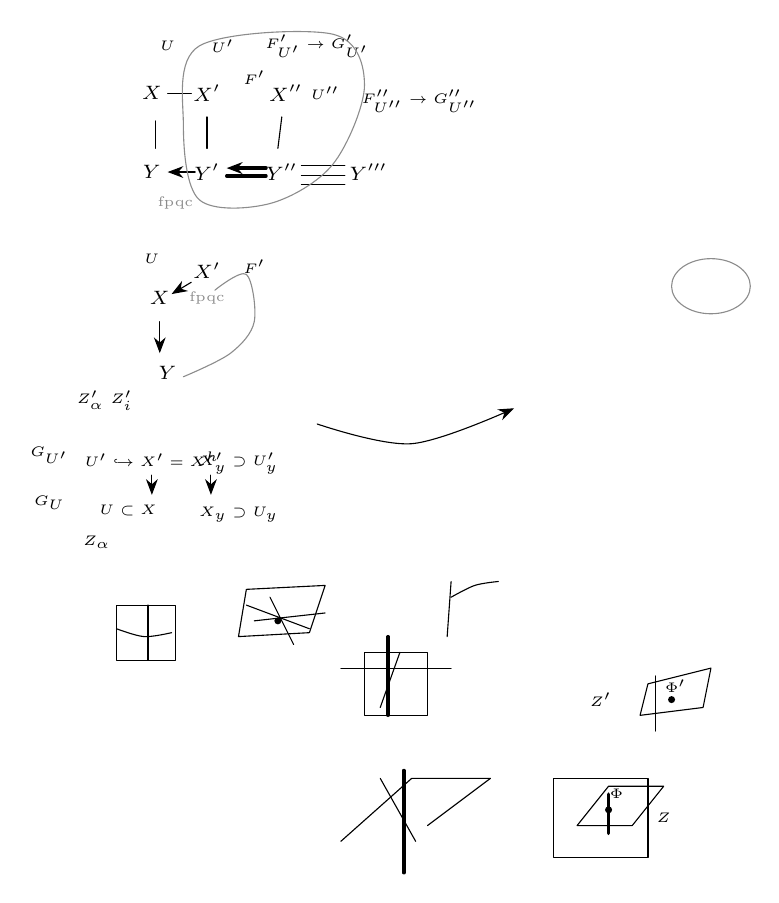
\begin{tikzpicture}[x=1mm,y=1mm,line cap=round,line join=round,font=\scriptsize]
\node[inner sep=1pt] at (24,-5) {\tiny $U$};
\node[inner sep=1pt] at (31,-5) {\tiny $U'$};
\node[inner sep=1pt] at (43,-5) {\tiny $F'_{U'}\to G'_{U'}$};
\node[inner sep=1pt] at (35,-9) {\tiny $F'$};
\node[inner sep=1pt] at (22,-11) {\scriptsize $X$};
\draw (24,-11) -- (27,-11);
\node[inner sep=1pt] at (29,-11) {\scriptsize $X'$};
\node[inner sep=1pt] at (39,-11) {\scriptsize $X''$};
\node[inner sep=1pt] at (44,-11) {\tiny $U''$};
\node[inner sep=1pt] at (56,-12) {\tiny $F''_{U''}\to G''_{U''}$};
\draw (22.5,-14.5) -- (22.5,-18);
\draw (29,-14) -- (29,-18);
\draw (38.5,-14) -- (38,-18);
\node[inner sep=1pt] at (22,-21) {\scriptsize $Y$};
\draw[-{Stealth[length=2mm]}] (27.5,-21) -- (24,-21);
\node[inner sep=1pt] at (29,-21) {\scriptsize $Y'$};
\draw[-{Stealth[length=2mm]},very thick] (36.5,-20.5) -- (31.5,-20.5);
\draw[very thick] (36.5,-21.5) -- (31.5,-21.5);
\node[inner sep=1pt] at (38.5,-21) {\scriptsize $Y''$};
\draw (41,-20.2) -- (46.5,-20.2);
\draw (41,-21.4) -- (46.5,-21.4);
\draw (41,-22.6) -- (46.5,-22.6);
\node[inner sep=1pt] at (49.5,-21) {\scriptsize $Y'''$};
\node[inner sep=1pt,pencil] at (25,-25) {\tiny fpqc};
\draw[pencil] plot[smooth cycle, tension=0.55] coordinates {(28,-5) (45,-3.5) (49,-10) (45,-20) (37,-25) (28,-24.5) (26,-15)};
\node[inner sep=1pt] at (22,-32) {\tiny $U$};
\node[inner sep=1pt] at (29,-33.5) {\scriptsize $X'$};
\node[inner sep=1pt] at (35,-33) {\tiny $F'$};
\draw[-{Stealth[length=2mm]}] (27,-35) -- (24.5,-36.5);
\node[inner sep=1pt] at (23,-37) {\scriptsize $X$};
\node[inner sep=1pt,pencil] at (29,-37) {\tiny fpqc};
\draw[-{Stealth[length=2mm]}] (23,-40) -- (23,-44);
\node[inner sep=1pt] at (24,-46.5) {\scriptsize $Y$};
\draw[pencil] plot[smooth, tension=0.55] coordinates {(30,-36) (34,-34) (35,-40) (32,-44) (26,-47)};
\node[inner sep=1pt] at (16,-50) {\tiny $Z'_\alpha\ Z'_i$};
\node[inner sep=1pt] at (9,-57) {\tiny $G_{U'}$};
\node[inner sep=1pt] at (22,-57.5) {\tiny $U'\hookrightarrow X'=X^h$};
\node[inner sep=1pt] at (33,-58) {\tiny $X'_y\supset U'_y$};
\draw[-{Stealth[length=2mm]}] (22,-59.5) -- (22,-62);
\draw[-{Stealth[length=2mm]}] (29.5,-59.5) -- (29.5,-62);
\node[inner sep=1pt] at (9,-63) {\tiny $G_U$};
\node[inner sep=1pt] at (19,-64) {\tiny $U\subset X$};
\node[inner sep=1pt] at (33,-64.5) {\tiny $X_y\supset U_y$};
\node[inner sep=1pt] at (15,-68) {\tiny $Z_\alpha$};
\draw[-{Stealth[length=2mm]}] plot[smooth, tension=0.55] coordinates {(43,-53) (55,-55.5) (68,-51)};
\draw[pencil] (93,-35.5) ellipse[x radius=5, y radius=3.5];
\draw (17.5,-76) -- (25,-76) -- (25,-83) -- (17.5,-83) -- cycle;
\draw (21.5,-76) -- (21.5,-83);
\draw plot[smooth, tension=0.55] coordinates {(17.5,-79) (21,-80) (24.5,-79.5)};
\draw (34,-74) -- (44,-73.5) -- (42,-79.5) -- (33,-80) -- cycle;
\draw (35,-78) -- (44,-77);
\draw (34,-76) -- (42,-79);
\draw (37,-75) -- (40,-81);
\node[pt] at (38,-78) {};
\draw (46,-84) -- (60,-84);
\draw (49,-82) -- (57,-82) -- (57,-90) -- (49,-90) -- cycle;
\draw[very thick] (52,-80) -- (52,-90);
\draw (53.5,-82) -- (51,-89);
\draw (60,-73) -- (59.5,-80);
\draw plot[smooth, tension=0.55] coordinates {(60,-75) (63,-73.5) (66,-73)};
\node[inner sep=1pt] at (79,-88) {\tiny $Z'$};
\draw (85,-86) -- (93,-84) -- (92,-89) -- (84,-90) -- cycle;
\node[pt] at (88,-88) {};
\node[inner sep=1pt] at (88.5,-86.3) {\tiny $\Phi'$};
\draw (86,-85) -- (86,-92);
\draw (46,-106) -- (55,-98) -- (65,-98) -- (57,-104);
\draw[very thick] (54,-97) -- (54,-110);
\draw (51,-98) -- (55.5,-106);
\draw (73,-98) -- (85,-98) -- (85,-108) -- (73,-108) -- cycle;
\draw (76,-104) -- (80,-99) -- (87,-99) -- (83,-104) -- cycle;
\draw[very thick] (80,-100) -- (80,-105);
\node[pt] at (80,-102) {};
\node[inner sep=1pt] at (81,-100) {\tiny $\Phi$};
\node[inner sep=1pt] at (87,-103) {\tiny $Z$};
\end{tikzpicture}
\end{document}
